% !TEX encoding = UTF-8
% !TEX program = lualatex

\documentclass[a4paper]{article}

\usepackage[left=1.5cm, right=1.5cm, top=1cm, bottom=2cm]{geometry}

\usepackage{mathtools, amssymb}
    \def\FF{\mathbf F}

\usepackage{fontspec}
    \setmainfont{Noto Serif}
    \setsansfont{Noto Sans TC}
    \setmonofont{Noto Sans Mono}

\usepackage{tikz}

\begin{document}

\parindent 0pt
\parskip 1em

\def\answersheet{}
\def\addblank#1{\xdef\answersheet{\answersheet#1}}
\newcounter{p}
\def\Problem#1{\stepcounter{p}[\thep]\addblank{[\thep]\hbox to#1{}\hskip0pt plus#1}}

\newcounter{c}
\def\choice#1{%
    \stepcounter{c}\ifnum\value{c}=27\setcounter{c}{1}\fi%
    #1(\Alph{c})\nobreak\ 
}
\def\no{\choice{}}
\def\yes{\choice{}}

\section*{Error Correcting Codes - Midterm Exam}

\sffamily

考試時間 Test time 09:30:00 am to 12:00:00 pm; 2.5 hours.
以教室投影機時鐘為準 Using the projected clock.
在答案卷作答 Answer on answer sheet.
每題一分 One point per problem.
全對才給分 No partial credit.
可以帶紙製品 Materials made of paper are allowed.
聽音樂請帶耳機 Use earphones for music.
禁止操作電子設備 Do not touch electronic devices.
助教不負責解釋題目 TA does not explain questions.
若題目怪怪的請仍盡力作答 Try your best even if a question looks wrong.

\rmfamily

$\FF_{4}$ is generated by 111 (i.e., $x^2 + x + 1$). \\
Its Zech table (i.e., $1 + \alpha^j = \alpha^{z(j)}$) is
0, 2, 1, 0.

$\FF_{8}$ is generated by 1011 (i.e., $x^3 + x + 1$). \\
Its Zech table (i.e., $1 + \alpha^j = \alpha^{z(j)}$) is
0, 3, 6, 1, 5, 4, 2, 0.

$\FF_{16}$ is generated by 10011 \\
(i.e., $x^4 + x + 1$).
Its Zech table is \\
0, 4, 8, 14, 1, 10, 13, 9, 2, 7, \\
5, 12, 11, 6, 3, 0.

$\FF_{64}$ is generated by 1011011 \\
(i.e., $x^6 + x^4 + x^3 + x + 1$).
Its Zech table is \\
0, 56, 49, 13, 35, 30, 26, 8, 7, 27, \\
60, 23, 52, 3, 16, 34, 14, 39, 54, 48, \\
57, 42, 46, 11, 41, 58, 6, 9, 32, 44, \\
5, 59, 28, 38, 15, 4, 45, 43, 33, 17, \\
51, 24, 21, 37, 29, 36, 22, 61, 19, 2, \\
53, 40, 12, 50, 18, 62, 1, 20, 25, 31, \\
10, 47, 55, 0.

$\FF_{128}$ is generated by 10000011 \\
(i.e., $x^7 + x + 1$).
Its Zech table is \\
0, 7, 14, 63, 28, 54, 126, 1, 56, 90, \\
108, 87, 125, 55, 2, 31, 112, 43, 53, 29, \\
89, 57, 47, 82, 123, 105, 110, 66, 4, 19, \\
62, 15, 97, 77, 86, 109, 106, 46, 58, 100, \\
51, 75, 114, 17, 94, 68, 37, 22, 119, 122, \\
83, 40, 93, 18, 5, 13, 8, 21, 38, 104, \\
124, 88, 30, 3, 67, 95, 27, 64, 45, 107, \\
91, 79, 85, 78, 92, 41, 116, 33, 73, 71, \\
102, 118, 23, 50, 101, 72, 34, 11, 61, 20, \\
9, 70, 74, 52, 44, 65, 111, 32, 117, 103, \\
39, 84, 80, 99, 59, 25, 36, 69, 10, 35, \\
26, 96, 16, 115, 42, 113, 76, 98, 81, 48, \\
121, 120, 49, 24, 60, 12, 6, 0.

\vskip-15cm
\leftskip10.5cm

$\FF_{32}$ is generated by 100101 \\
(i.e., $x^5 + x^2 + 1$).
Its Zech table is \\
0, 18, 5, 29, 10, 2, 27, 22, 20, 16, \\
4, 19, 23, 14, 13, 24, 9, 30, 1, 11, \\
8, 25, 7, 12, 15, 21, 28, 6, 26, 3, \\
17, 0.

$\FF_{256}$ is generated by 100011101 \\
(i.e., $x^8 + x^4 + x^3 + x^2 + 1$).
Its Zech table is \\
0, 25, 50, 223, 100, 138, 191, 112, 200, 120, \\
21, 245, 127, 99, 224, 33, 145, 68, 240, 92, \\
42, 10, 235, 196, 254, 1, 198, 104, 193, 181, \\
66, 45, 35, 15, 136, 32, 225, 179, 184, 106, \\
84, 157, 20, 121, 215, 31, 137, 101, 253, 197, \\
2, 238, 141, 147, 208, 63, 131, 83, 107, 82, \\
132, 186, 90, 55, 70, 162, 30, 216, 17, 130, \\
64, 109, 195, 236, 103, 199, 113, 228, 212, 174, \\
168, 160, 59, 57, 40, 170, 242, 167, 175, 203, \\
62, 209, 19, 158, 202, 176, 251, 190, 139, 13, \\
4, 47, 221, 74, 27, 248, 39, 58, 161, 71, \\
126, 246, 7, 76, 166, 243, 214, 122, 164, 153, \\
9, 43, 117, 183, 180, 194, 110, 12, 140, 239, \\
69, 56, 60, 250, 177, 144, 34, 46, 5, 98, \\
128, 52, 218, 150, 135, 16, 217, 53, 206, 188, \\
143, 178, 226, 119, 201, 159, 169, 41, 93, 155, \\
81, 108, 65, 182, 118, 227, 114, 87, 80, 156, \\
85, 211, 229, 232, 79, 88, 95, 134, 151, 37, \\
124, 29, 163, 123, 38, 249, 61, 204, 149, 219, \\
97, 6, 247, 28, 125, 72, 23, 49, 26, 75, \\
8, 154, 94, 89, 187, 207, 148, 205, 54, 91, \\
241, 171, 78, 233, 116, 44, 67, 146, 142, 189, \\
252, 102, 237, 3, 14, 36, 152, 165, 77, 172, \\
231, 230, 173, 213, 244, 22, 73, 222, 51, 129, \\
18, 210, 86, 115, 234, 11, 111, 192, 105, 185, \\
133, 96, 220, 48, 24, 0.

\leftskip0cm

\vskip-1.5cm

\[\begin{tikzpicture} [overlay, rotate=90, yshift=0.5cm]
    \draw (0, 0) -- (10, 0);
    \foreach \x in {0, ..., 9} {
        \pgfmathtruncatemacro\xa{floor(\x / 10)}
        \pgfmathtruncatemacro\xb{mod(\x, 10)}
        \draw (\x, 0) -- +(0, 0.3) node [left] {$\xa.\xb$};
        \draw (\x.5, 0) -- +(0, 0.2);
        \foreach \y in {1, ..., 9} {
            \draw (\x + \y/10, 0) -- +(0, 0.1);
        }
    }
     \foreach \k in {1, ..., 9} {
        \draw ({10 * log10(\k)}, 0) -- +(0, -0.3)
            node [right] {$\log_{10}\k$};
        \draw ({10 * log10(\k + 0.5)}, 0) -- +(0, -0.2);
        \foreach \l in {1, 2, 3, 4, 6, 7, 8, 9} {
            \draw ({10 * log10(\k + 0.\l)}, 0) -- +(0, -0.1);
        }
    }
\end{tikzpicture}\]

For questions with precision requirements,
(2x) means that your answer should be in $[a/2, 2a]$,
(5x) means  $[a/5, 5a]$.
For this kind of questions, answer in scientific notation such as 1.2e345.

% \section{Code Meta}

\Problem{2em}
A symbol is the basic unit in the context of error-correcting codes;
it corresponds to which basic unit in linear algebra?
\no a basis
\no a vector
\no a linear subspace
\yes a finite field element

\Problem{2em}
Because the theory of error-correcting codes
is closely related to linear algebra,
a codeword is quite often used interchangeably with
which of the following terminologies?
\no a basis
\yes a vector
\no a linear subspace
\no a finite field element

\Problem{2em}
The alphabet size is very crucial in coding theory
as MDS codes and near-MDS codes are easier to construct
when the alphabet size is larger.
Among the following choices, which one do you think
is the most probable notation that can be interpreted as the alphabet size?
\no $n$
\no $k$
\no $d$
\yes $|F|$ 

\Problem{2em}
In literature, the code rate is sometimes
not an independent variable, i.e., it can be expressed by other quantities.
Assuming the usual notation in coding theory as well as in this course,
which of the following is most likely the expression of the code rate?
\yes $k/n$
\no $d/n$
\no $k \log_2 |F|$
\no $\log_{|F|} n$

\Problem{2em}
When discussing a family of codes,
it is not favorable to talk about the absolute distance
because it varies from code to code.
However, for certain applications,
the relative distance might tend to a fixed constant,
making them a parameter worth studying.
When there is only one code, nevertheless,
how would you express the relative distance?
\no $k/n$
\yes $d/n$
\no $k \log_2 |F|$
\no $\log_{|F|} n$

\Problem{2em}
By the work of Shannon, we know that
codes with larger and larger block lengths
achieve Shannon capacity.
But this doesn't mean that we should use very large block lengths
because of latency and decoding complexity.
To quantify how many message bits are transmitted per block so that
we can infer how much latency we are going to bear, it is expressed as?
\no $k/n$
\no $d/n$
\yes $k \log_2 |F|$
\no $\log_{|F|} n$

% \section{Popular codes}

\Problem{3em}
Linear codes is widely studied in coding theory
because of several nice properties.
Among the given choices, select as many linear codes as possible.
\yes cyclic code
\yes repetition code
\no tension product code

\Problem{3em}
Here are some closely related codes.
Select exactly the ones that are linear codes.
\no singleton code
\yes single parity-check code
\yes low-density parity-check code

\Problem{3em}
You are given several choices.
Your job is to select one or more choices such that the select choices
are all linear codes and none of the unselected choices is a linear code.
\yes Hamming code
\no Muller--Solomon code
\no Bose--Chiwawa--Hondatomato code

\Problem{4em}
In class, we introduce an exceptional family of codes whose codewords can be,
and should be, arranged as 2D matrices.
In class, we comment that decoding such codes looks like a <noun> puzzle.

\Problem{4em}
We also introduce evaluation codes in class.
Among them there is a binary one and a non-binary one.
The binary one evaluates <adjective> polynomials,
where <adjective> also appears in the mock exam.

\Problem{4em}
What about the non-binary one?
It evaluates <adjective> polynomials,
enjoys the MDS property,
and finds applications in, e.g., QR codes.

% \section{Linear Algebra}

\Problem{4em}
The entries of the following matrix are in $\FF_2$.
What are the parameters $[n, k, d]$
when the matrix is treated as the $G$ of some error-correcting code?
\[
    \setcounter{MaxMatrixCols}{12}
    \begin{bmatrix}
        0 & 0 & 0 & 0 & 0 & 0 & 1 & 1 & 1 & 1 & 1 & 1 \\
        1 & 0 & 1 & 0 & 1 & 0 & 1 & 0 & 1 & 0 & 1 & 0 \\
        1 & 1 & 0 & 1 & 1 & 0 & 1 & 1 & 0 & 1 & 1 & 0 \\
    \end{bmatrix}
\]

\Problem{10em}
The weight enumerator of a code
is an essential tool used to study its performance.
It not only captures the minimal distance of the code, but it also
gives the ``coefficient'' in the frame error rate approximation.
What is its weight enumerator (as a polynomial in $X$)
of the code generated by the $G$ above?

\Problem{10em}
An information set is a subset of columns such that,
when the corresponding symbols are not erased,
the entire codeword can be recovered,
while erasing even one more symbol makes the recovery impossible.
List all information sets containing the first two columns
of the $G$ discussed above.

\Problem{10em}
An information set can also be defined
as a subset of columns such that
isolating these columns and deleting all other columns
leads to a square matrix that is invertible.
List all information sets that
do not use the first two columns and
do not use neighboring columns
(that is, column $j$ and column $j + 1$ cannot both be used).
(There are about 13 answers.)

\Problem{10em}
What is the $H$ corresponding to this $G$?
Note that $H$ is not unique.
So make the top rows of $H$ the identity matrix
(this is called the systematic form)
and answer the bottom part of $H$.

\Problem{10em}
Consider the code generated by the $G$ above.
Shortening a code at the first column means that
we are interested in codewords whose first entry is zero.
Find a generator matrix of the shortened code,
with the first column removed because we all know it is all zero.
Then find the rref form of the matrix by row operations
(but no column permutation, i.e., no pivoting).

\Problem{5em}
What is the smallest Reed--Muller code containing the codeword below?
Answer the parameters $(r, m)$ and $[n, k, d]$.
Note that I did not specify which directions are $x$, $y$, and $z$.
But it does not matter, because Reed--Muller codes are invariant
under variable permutations.
In fact, it is invariant under a larger group of automorphisms:
the affine group.
\[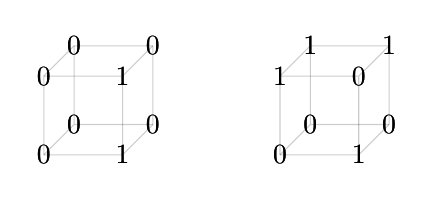
\begin{tikzpicture}
    \foreach \a in {0, 1} {
        \tikzset{xshift=\a * 3cm}
        \foreach \x in {0, 1} {
            \foreach \y in {0, 1} {
                \draw [opacity=0.2]
                    (\x, \y, 0) -- (\x, \y, 1)
                    (\y, 0, \x) -- (\y, 1, \x)
                    (0, \x, \y) -- (1, \x, \y)
                ;
                \foreach \z in {0, 1} {
                    \foreach \w in {0, 1} {
                        \pgfmathtruncatemacro\eval
                        {mod(\x * \z + \y * \a, 2)}
                        \draw (\x, \y, \z) node {$\eval$};
                    }
                }
            }
        }
    }
\end{tikzpicture}\]

\Problem{5em}
What is the smallest Reed--Muller code containing the codeword below?
Answer the parameters $(r, m)$ and $[n, k, d]$.
\foreach \a in {0, 1} {
    \[\begin{tikzpicture}
        \foreach \b in {0, 1} {
            \tikzset{xshift=\b * 3cm}
            \foreach \x in {0, 1} {
                \foreach \y in {0, 1} {
                    \draw [opacity=0.2]
                        (\x, \y, 0) -- (\x, \y, 1)
                        (\y, 0, \x) -- (\y, 1, \x)
                        (0, \x, \y) -- (1, \x, \y)
                    ;
                    \foreach \z in {0, 1} {
                        \foreach \w in {0, 1} {
                            \pgfmathtruncatemacro\eval
                            {mod(1 + \z*(1-\x) + (1-\a)*\b + \y*\z*\a*\b, 2)}
                            \draw (\x, \y, \z) node {$\eval$};
                        }
                    }
                }
            }
        }
    \end{tikzpicture}\]
}

\Problem{6em}
What is the generator polynomial of the
smallest cyclic code containing $01011100110100$?
Note that one can interpret 1011 as $x^3 + x + 1$ or $1 + x^2 + x^3$.
But either way the answer is unique if it is written down as a binary string.
The high--low degree distinction is not important here;
what matters is the left--right direction.

\Problem{6em}
The first row of $H$ is $0001$ and the last row is $1111$.
Between them are binary representations of $2$--$14$.
Correct the received word $111110000011111$ that is flipped at most once.

\Problem{3em}
A rateless code is used to protect $3$ bits: $a$, $b$, and $c$.
Seven linear combinations are sent periodically:
$a$, $a + b$, $b$, $b + c$, $a + b + c$, $a + c$, $c$.
The erasure pattern is nnnynnnynnnynnny ... (three nos one yes).
How many symbols are sent before the receiver can decode all three bits?

% \section{Finite Field}

\Problem{10em}
List the sizes of all finite fields from $20$ to $40$.

\Problem{6em}
Find one irreducible polynomial of degree $9$ over $\FF_2$.

\Problem{6em}
Find one irreducible polynomial of degree $5$ over $\FF_3$.

\Problem{10em}
Use the polynomial representation (you can say 1001 instead of $x^3 + 1$)
to reproduce the addition table of $\FF_8$ on the answer sheet.

\Problem{10em}
Use the polynomial representation (you can say 1001 instead of $x^3 + 1$)
to reproduce the division table of $\FF_8$ on the answer sheet.

\Problem{10em}
Use the Zech-logarithm representation
to reproduce the addition table of $\FF_8$ on the answer sheet.

\Problem{10em}
Use the Zech-logarithm representation
to reproduce the division table of $\FF_8$ on the answer sheet.

\Problem{10em}
What is the most natural $G$ of the $[7, 3]$ Reed--Solomon code over $\FF_7$?
(Row operations on $G$ does not change the code.
But there is a special $G$ that aligns with the narrative.)

\Problem{4em}
A BCH code with designed roots $\alpha, \alpha^2, \alpha^3$ is used,
where $\alpha$ is the generator of $\FF_{256}$.
A received word $r$ is such that
$r(\alpha) = \alpha^{249}$ and $r(\alpha^3) = \alpha^{67}$.
Find the error-locating polynomial $aX^2 + bX + c$.

\Problem{4em}
The polynomial is said to be error-locating
because its roots reveal the locations of the errors.
Usually, having $\alpha^j$ as a root means that the error is at position $j$.
Solve the error-locating polynomial above.

% \section{Combinatorics}

\Problem{3em} (2x)
For the $[7, 3]$ Reed--Solomon over $\FF_7$,
how many codewords have distinct symbols?
There is a clever trick that can find the exact answer,
but since a roughly estimated is also acceptable,
you can simply sample a couple of codewords and extrapolate the answer.
It is the same idea of counting the number of fish in a lake
by catching, tagging, and releasing.

\Problem{3em} (2x)
Consider a tensor product code whose codewords are
$30 \times 30$ binary matrices whose rows and columns sum to even numbers.
How many codewords have weight $6$?
It is possible to express this answer using multiple binomial coefficients.
But I want that the answer is in scientific notation.
So please evaluate all the binomial coefficients.

\Problem{3em} (2x)
Consider a tensor product code whose codewords are
$10 \times 10 \times 10$ binary cubes whose ``3D-rows''
(ten collinear entries parallel to the X, Y, or Z axis)
sum to even numbers.
How many codewords have weight $6$?
Again, this problem can be solved exactly using binomial coefficients.
But I want scientific notation.

\Problem{3em} (2x)
The corresponding trellis of a turbo code
has four rows and five columns.
From one column to the next, only $+0, +1$ are allowed.
The code is used over an erasure channel.
How many erasure patterns are such that
the decoder cannot recover the message correctly?

% \section{Probability}

\Problem{3em} (2x)
If a Wi-Fi environment is such that
every $1$ KiB of data has an error probability of $10^{-8}$,
what is the probability that a $1$-GiB file contains at least one error?
Note that some brands use 1 KB = 1000 bytes instead of 1024 bytes
to confuse customers.
That is why the middle-i version, KiB, MiB, GiB, etc, is introduced.
However, for these questions,
I don't think it matters that much which definition you use.

\Problem{3em} (2x)
What is the new probability if every KiB is protected by a parity-check bit
and resent until the parity check matches?
As you might have already guessed,
there are many ways to interpret how the parity check is added.
For instance it can be $n = 1024$ or $k = 1024$.
But does it matter?

\Problem{3em} (2x)
What is the capacity of the binary symmetric channel
with crossover probability $10^{-2}$?

\Problem{3em} (2x)
What is the frame error rate if the Hamming code
of length $7$ is used over the BSC above?

\Problem{3em} (2x)
Now the code above is used to protect the symbols
of an $[14, 10]$ RS code over $\FF_{128}$.
What is the frame error rate?

\Problem{3em} (2x)
BPSK is used over AWGN with $\sigma = 0.1$.
Three symbols whose product is $1$ are sent.
What is frame error rate?

\Problem{3em} (2x)
16-QAM is used over a pair of AWGN channels
(one for the real part and one for the imaginary part) with $\sigma = 0.1$.
A signal $s$ such that $\Re s, \Im s \in \{-1.5, -0.5, 0.5, 1.5\}$ is sent,
and $1 + 1i$ is received.
What is the posterior probability of $s = -1.5 - 1.5i$?

\Problem{3em} (2x)
What is the posterior probability of $s = -0.5 -0.5i$?

% \section{Relevant Knowledge}

\Problem{3em} (5x)
At 120 Hz refresh rate, how much data (bits per second)
is transmitted over HDMI for a 1920x1080 display with 24-bit colors?

\Problem{3em} (5x)
What is the largest QAM modulation Wi-Fi 6 supports?

\Problem{3em} (5x)
How much RAM does iPhone 17 Pro Max have?

\Problem{3em} (5x)
How many FLOPS can GeForce RTX 5090 deliver
for single-precision (FP32) operations?

\Problem{3em} (5x)
How much data does the large hadron collider (LHC) generate each year?

\cleardoublepage

\section*{Error Correcting Codes - Midterm Exam}

\parskip0pt
\advance\lineskip1cm plus1fil
\advance\baselineskip1cm plus1fil

Name (zh or en) \hfil Student ID

\answersheet

\end{document}